\label{section:XPS}\index{XPS} 
\textbf{X}-Ray \textbf{p}hotoelectron \textbf{s}pectroscopy (XPS) is a tool to achieve information of the samples chemical structure.
When X-rays with sufficient energy hit metals, electrons are emitted. This effect is called photoelectric effect and was first discovered by Heinrich Hertz in 1887 through the fact that electrodes illuminated with ultraviolet light create electric sparks more easily. \cite{hertz_ueber_1887} 18 years later Albert Einstein received the Nobel Price for his discovery of the law of the photoelectric effect\cite{_nobel_prize_1921} and a scientific explanation which Hertz was missing. The emitted electron's kinetic energy depends on the element the electron was emitted from and allows for exact identification of the atomic species on the sample that is used in a wide field of investigations and awarded Kai M. Siegstein with a nobel prize in 1981\cite{_noble_price_1981}.

\subsection{Theory}
\index{XPS!Physical model}As the X-rays hit and penetrate the sample surface they excite electrons and initiate core-level excitations.

For the \textbf{core-level excitation} the X-ray removes a single electron strongly bound to the core. Energy conservation due to elastic scattering of the electron out of the bulk results in the relation 
\begin{align}
%E_{kin} &= h\nu_{\textnormal{X-ray}}-E_{B}-\Phi_{\textnormal{analyzer}} \\
E_B 	&=h\nu_{\textnormal{X-ray}}-E_{kin}-\Phi_{\textnormal{analyzer}}
\end{align}
 $h\nu_{\textnormal{X-ray}}$ is the energy of the incident X-ray beam, $E_B$ the binding energy of the excited electron and $\Phi_{analyzer}$ the work function of the analyzer. The stronger the binding energy, the less energy is left for kinetic energy.


\begin{figure}\centering
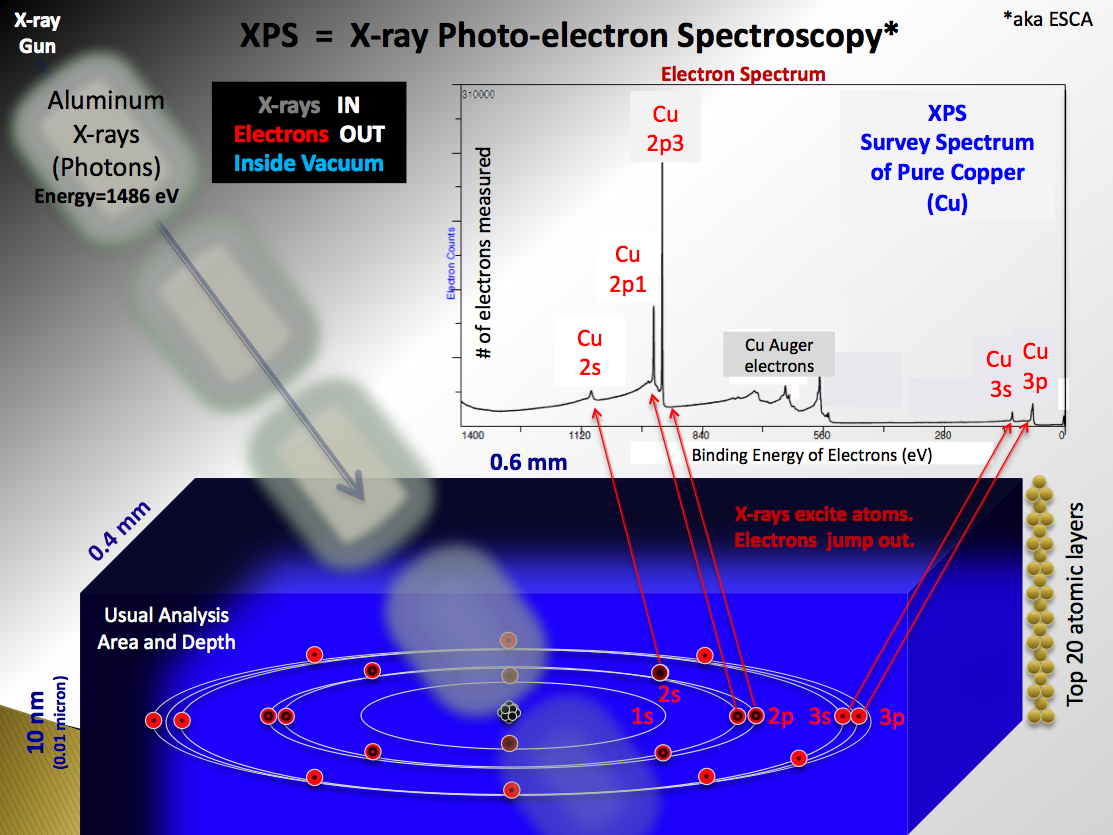
\includegraphics[width=0.7\textwidth]{./images/XPS_PHYSICS}
		\label{fig:XPS-excitation}
	\caption{Representation of a XPS process. A scheme of a X-ray gun illuminating a sample area of about \SI{0.4}{\milli \meter} $\times$ \SI{0.6}{\milli \meter} is shown. X-rays are used to excite core level electrons. Excited electrons within the first 20 layer escape the sample. After leaving the sample these show element specific signatures in their kinetic energies. A detailed analysis of the peak shift allows for identification of the chemical environment.}
	\label{fig:auger-core}
\end{figure}

\cite{zemlyanov_versatile_2018}
The \index{XPS!chemical surrounding} \textbf{chemical surrounding} of atoms changes their binding energy, making XPS an ideal tool to detect changes in chemical surrounding. Although the analysis is averaged over the area of the incident X-rays its results are very precise. This makes it possible to distinguish differently bound atoms within single atomic species and therefore gives rise to otherwise not directly observable processes like growth, intercalation, etching and binding of for example 
graphene islands on Ir(111)\cite{busse_graphene_2011-1,granas_oxygen_2012}.
The \index{XPS!binding energies} binding energies of some atomic transitions are given in \autoref{tab:XPS-intensities}.

\begin{table}\centering
 \caption{Element specific transitions and binding energies for some chosen elements as reported in \cite{wanger_handbook_1979}}
 \begin{tabular}{lll}
  Element & Ground state & $E_B$ [eV]\\ \hline 
  O & 1s & 531\\
  N & 1s & 398.1\\
  C & 1s & 285\\
  B & 1s & 189.4 \\
%  Cu & 2p $\frac{1}{2} (\frac{3}{2})$ & 953 (933) \\
%  Cu & LMM & 560-580 \\
  Cu & 3s & 123\\
  Cu & 3p $\frac{1}{2} (\frac{3}{2})$ & 77 (75)\\
 \end{tabular}
\label{tab:XPS-intensities}
\end{table}

The shape of the peaks typically resembles the line shape of the used X-rays (Gauss width $\approx 1eV$). In case of s-states $(l=0)$ (B\textit{1s}, N\textit{1s}, C\textit{1s}) the peaks are singlets. With increasing $j=l+s$, the spin-orbit (j-j) coupling introduces a 'parallel' and 'anti-parallel' nature of the spin, resulting in two different $j=\frac{1}{2}(\frac{3}{2})$ and therefore two different energies.
% The split in energy is expected to increase with the atomic number Z (for constant n,l) or as l decreases (n constant). This makes the splitting of 3p orbitals larger than that of the 3d's. 
The ratio of the two peaks is given by their degeneracy $(2j+1)$\cite[113]{Riviere_90}, so that the $\textnormal{Cu3p}\frac{3}{2}$ peak is two times larger than $\textnormal{Cu3p}\frac{1}{2}$.

\subsection{Experimental details}
The \textbf{X-ray sources} used are supplied with aluminum and magnesium anodes.
%\footnote{Other materials are available that produce various X-ray energies and line widths \index{XPS!Anode materials} \cite{_x-ray_2015}.} 
With these, electrons are accelerated with typically \SI{15}{\keV} onto the anode of choice. Most of the created radiation is made up of the principal characteristic line ($K\alpha_{1,2}$). Higher ones ($K\alpha_{3,4}$, $K\beta$) are also observed but with much lower intensities. In addition there is a continuous background called Bremsstrahlung extending up to the energy of the incident electron energy. This background is of no use for the XPS measurement and has to be subtracted in a more or less artificial way. For XPS measurements the Mg K$\alpha$ = \SI{1253.6}{\eV} and Al K$\alpha$ = \SI{1486.6}{\eV} are used situationally to shift the core level spectra with respect to substrate transitions (Auger transitions) at constant kinetic energy.

The more atoms of a specific kind are present, the larger the signal gets. Therefore the signal intensity resembles the amount of atoms on the topmost surface layers($\approx \SI{10}{\nm}$). As each irradiated atomic species has a different \textbf{cross section} for adsorption of X-rays with a certain energy they emit spectra with a different intensity. Comparing the cross section of e.g. N and B, one can see that it it roughly 4 times as large (B: \SI{6,87e3}{\barn\per atom}, N: \SI{25,82e3}{\barn\per atom}) for $\textnormal{Al} K_{\alpha}$\cite{henke_x-ray_1993}. Meaning that the signal from the N is much stronger than that of the B, although their number of atoms is equal.

\textbf{Gracing and normal emission} are two operational modes in XPS. The maximum information depth in XPS measurements is mainly limited by the escape length of excited core level electrons ($\approx \SI{10}{\nano \meter}$). The mean free path of electrons with energy E in a solid is approximated by $\lambda = \frac{143}{E^2} + 0.054 \sqrt{E} \stackrel{E=\SI{1}{\kilo \eV}}{\approx} \SI{1.7}{\nano \meter}$.\cite{Seah_Quantitative_1979} This is much smaller than the penetration depth of X-Rays which are in the order of \SI{10}{\nano \meter}. An increasing angle between sample and detector increases the path the electrons have to travel through the bulk to reach the analyzer. Because the mean free path of the electrons stays the same, a longer route in the bulk attenuates the signal of lower lying substrate atoms. Electrons leaving the surface adsorbate are not attenuated and gain in signal strength relative to the bulk atoms.

Some supporting measurements are done in gracing emission to increase an otherwise small signal of an surface adsorbate but are not shown in this work.

The spectra used in this work are recorded without monochromator. Experiments are done at two different XPS setups. (1) The RT-STM/XPS (2) The NIM-XPS chamber.  

\subsection{Limitations}
\paragraph{Beam damage}
Since the X-Rays carry considerable energy other effects than the excitation of core electrons are possible. Especially for long integration times of the analyzer (for elements with little cross section or little surface coverage) the amount of deposited energy results in unwanted side reactions on the surface. It is possible to trigger a change in the chemical surrounding of the investigated element, causing chemical shifts that are not present in the pristine sample and change the XPS spectrum over time.

\paragraph{Space averaging technique}
XPS is a space averaging technique. First the X-Ray beam has an inherent width, the analysis area can't be chosen arbitrarily small. Second, X-Rays do excite electrons not only directly within the illuminated area, but penetrate the bulk and cause a cascade of transitions in the sample. The resulting information is always a mix between surface adsorbates and bulk elements.